%!TEX TS-program = PdfLaTeX
%!TEX encoding = UTF-8 Unicode


\documentclass[xcolor=x11names, compress, 11pt]{beamer}
% Options for doc
    % handout to hide navigation bar
    % compress to make slide content compressed


\mode<presentation>


%%%%%%%%%%%%%%%%%%%%%%%%%%%%%%% Define new colors %%%%%%%%%%%%%%%%%%%%%%%%%%%%%%
\definecolor{Amaranth}{rgb}{0.9, 0.17, 0.31}
\definecolor{Asparagus}{rgb}{0.53, 0.66, 0.42}
\definecolor{Amber}{rgb}{1.0, 0.49, 0.0}
\definecolor{emphase}{rgb}{0.9, 0.17, 0.31}
\definecolor{BrownGreen}{HTML}{586E75}

\definecolor{SolarizedViolet}{HTML}{6c71c4}
\definecolor{SolarizedMagenta}{HTML}{d33682}
\definecolor{SolarizedBlue}{HTML}{268bd2}
\definecolor{SolarizedCyan}{HTML}{2aa198}
\definecolor{SolarizedGreen}{HTML}{859900}
\definecolor{SolarizedRed}{HTML}{dc322f}
\definecolor{BeeYellow}{HTML}{ffcb00}
\definecolor{SolarizedOrange}{HTML}{cb4b16}
\definecolor{SolarizedYellow}{HTML}{b58900}

\definecolor{SolarizedWhite}{HTML}{fdf6e3}
\definecolor{SolarizedBrWhite}{HTML}{eee8d5}
\definecolor{SolarizedBrCyan}{HTML}{93a1a1}
\definecolor{SolarizedBrBlue}{HTML}{839496}
\definecolor{SolarizedBrYellow}{HTML}{657b83}
\definecolor{SolarizedBrGreen}{HTML}{586e75}
\definecolor{SolarizedBlack}{HTML}{073642}
\definecolor{SolarizedBrBlack}{HTML}{002b36}
\definecolor{ClassicBlack}{HTML}{000000}



%%%%%%%%%%%%%%%%%%%%%%%%%%%%%%%%%%% Packages %%%%%%%%%%%%%%%%%%%%%%%%%%%%%%%%%%%
\usepackage[OT1, T1]{fontenc}                              % .pdf Encoding spec
\usepackage[utf8]{inputenc}                                % .tex Encoding spec
\usepackage[autostyle=true, threshold=0]{csquotes}         % Ensure correct quote text even nested one
\usepackage[greek, french]{babel}                          % language used
\usepackage{palatino}                                      % Font used
\usepackage{graphicx}                                      % Add images

\usepackage{hyperref}
\hypersetup{
      pdfauthor   = {Jérémy Bois},%
      pdftitle    = {Soutenance - Outil d’Aide à la Décision pour la Conception de Maisons Solaires à Énergie Positive},%
      pdfsubject  = {Soutenance Thèse - 20171009},%
}


\usepackage{color, colortbl, transparent}             % Add colors and opacity

\usepackage[separate-uncertainty=true,%
            per-mode=symbol]{siunitx}                 % Unit package
\usepackage{amsmath, amssymb, amsthm, mathtools,bm}   % Allow adding complex equations
% \usepackage{nicefrac}                               % for \nicefrac macro
% \usepackage{letltxmacro}                            % Support for optional argument in redefinition

\sisetup{output-decimal-marker={,}}                   % ... and in siunitx: dot with comma
% Writing a dot print a comma in math mode
\mathchardef\period=\mathcode`.                       % Allows to still write a dot if needed
\DeclareMathSymbol{.}{\mathord}{letters}{"3B}         % Decimal separator in math mode ...


\makeatletter % changes the catcode of @ to 11
    % Sign function
    \DeclareMathOperator{\sign}{sign}

    % Change the ways square root appears
    \let\oldr@@t\r@@t
    \def\r@@t#1#2{%
    \setbox0=\hbox{$\oldr@@t#1{#2\,}$}\dimen0=\ht0
    \advance\dimen0-0.1\ht0
    \setbox2=\hbox{\vrule height\ht0 depth -\dimen0}%
    {\box0\lower0.59pt\box2}}
    \LetLtxMacro{\oldsqrt}{\sqrt}
    \renewcommand*{\sqrt}[2][\ ]{\oldsqrt[#1]{#2}}

    % Quick and easy way to typeset abs (|) and norm (||)
    \DeclarePairedDelimiter\abs{\lvert}{\rvert}
    % Swap the definition of \abs* and \norm*, so that \abs and \norm resizes the
    % size of the brackets, and the starred version does not.
    \let\oldabs\abs
    \def\abs{\@ifstar{\oldabs}{\oldabs*}}
\makeatother % changes the catcode of @ back to 12


\usepackage{booktabs, multirow}                            % Easy pro tables and multiple row
% New columns type
\newcolumntype{B}{>{\columncolor{Amaranth}}c}
\newcolumntype{G}{>{\columncolor{Asparagus}}c}
\newcolumntype{R}{>{\columncolor{Amber}}c}


\usepackage{changepage}                                    % Enable changing text margins
\usepackage{tikz,tcolorbox}





%%%%%%%%%%%%%%%%%%%%%%%%%%%%%%%%% Beamer Layout %%%%%%%%%%%%%%%%%%%%%%%%%%%%%%%%
% Head with sections
\useoutertheme[subsection=false, shadow]{miniframes}
\useinnertheme{default}
\usefonttheme{professionalfonts}
\usefonttheme{serif}

\setbeamerfont{title like}{shape=\scshape}
\setbeamerfont{frametitle}{shape=\scshape}

\setbeamercolor{bgcolor}{fg=black,bg=blue}
\setbeamercolor{lower separation line head}{bg=SolarizedBlue}
\setbeamercolor{frametitle}{fg=SolarizedBlue,bg=SolarizedBrWhite}
\setbeamercolor{title}{fg=SolarizedBlue,bg=SolarizedBrWhite}
\setbeamercolor{normal text}{fg=ClassicBlack,bg=white}
\setbeamercolor{alerted text}{fg=SolarizedRed,bg=SolarizedBrWhite}
\setbeamercolor{example text}{fg=ClassicBlack}
\setbeamercolor{structure}{fg=ClassicBlack}
\setbeamercolor{palette tertiary}{fg=ClassicBlack,bg=black!10}
\setbeamercolor{palette quaternary}{fg=ClassicBlack,bg=black!10}
\setbeamercolor{footlinecolor}{fg=DeepSkyBlue4,bg=black!10}

\setlength\fboxsep{0pt}
\setlength\fboxrule{0.5pt}

% Remove navigation symbols
\setbeamertemplate{navigation symbols}{}

% Complete footline with small caps for subsection name
\setbeamertemplate{footline}{%
  \begin{beamercolorbox}[sep=1em,wd=\paperwidth,leftskip=0.5cm,rightskip=0.5cm]{footlinecolor}
    \tiny
    \hfill \textsc{\small\textbf{\insertsubsection}}\hfill \insertframenumber{} / \inserttotalframenumber
    \hfill
  \end{beamercolorbox}%
}




%%%%%%%%%%%%%%%%%%%%%%%%%%%%%%%%% Specific Layout %%%%%%%%%%%%%%%%%%%%%%%%%%%%%%
\setbeamertemplate{title page}{%
  \vbox{}
  \begingroup
    \centering
    \begin{beamercolorbox}[sep=8pt,center,shadow=true,rounded=true]{title}
      \usebeamerfont{title}\inserttitle\par%
      \ifx\insertsubtitle\@empty%
      \else%
        \vskip0.25em%
        {\usebeamerfont{subtitle}\usebeamercolor[fg]{subtitle}\insertsubtitle\par}%
      \fi%
    \end{beamercolorbox}%
    \vskip1em\par
    \begin{beamercolorbox}[sep=8pt,center]{author}
      \usebeamerfont{author}\insertauthor
    \end{beamercolorbox}
    % \begin{beamercolorbox}[sep=8pt,center]{institute}
    %   \usebeamerfont{institute}\insertinstitute
    % \end{beamercolorbox}
    \begin{beamercolorbox}[sep=8pt,center]{date}
      \usebeamerfont{date}\insertdate
    \end{beamercolorbox}
  \endgroup
  \vfill
}


% Before each section
\AtBeginSection[]
{
 \begin{frame}[plain]
  \vfill
  \centering
  \begin{beamercolorbox}[sep=8pt,center,shadow=true,rounded=true]{title}
    \usebeamerfont{title}\insertsectionhead\par%
  \end{beamercolorbox}
  \vfill
  % \addtocounter{page}{-1}
  \end{frame}
}




%%%%%%%%%%%%%%%%%%%%%%%%%%%%%%%%% Custom commands %%%%%%%%%%%%%%%%%%%%%%%%%%%%%%
% Add boxed subtitle
\newcommand{\addsubtitle}[1]{%
\begin{beamercolorbox}[sep=2pt,center,shadow=true,rounded=true]{footlinecolor}
    #1\par%
\end{beamercolorbox}%
}

% Add boxed alert
\newcommand{\addalert}[1]{%
\begin{beamercolorbox}[sep=2pt,center,shadow=true,rounded=true]{alerted text}
    #1\par%
\end{beamercolorbox}%
}

% Add smileys
\newcommand{\addSimley}[2]{%
\begin{tikzpicture}[scale=0.11]
    \newcommand*{\SmileyRadius}{1.5}%
    \draw [fill=#2] (0,0) circle (\SmileyRadius)% outside circle
        %node [yshift=-0.22*\SmileyRadius cm] {\tiny #1}% uncomment this to see the smile factor
        ;

    \pgfmathsetmacro{\eyeX}{0.5*\SmileyRadius*cos(30)}
    \pgfmathsetmacro{\eyeY}{0.5*\SmileyRadius*sin(30)}
    \draw [fill=SolarizedBrBlack,draw=none] (\eyeX,\eyeY) circle (0.2cm);
    \draw [fill=SolarizedBrBlack,draw=none] (-\eyeX,\eyeY) circle (0.2cm);

    \pgfmathsetmacro{\xScale}{2*\eyeX/180}
    \pgfmathsetmacro{\yScale}{1.0*\eyeY}
    \draw[color=SolarizedBrBlack, domain=-\eyeX:\eyeX]
        plot ({\x},{
            -0.1+#1*0.15 % shift the smiley as smile decreases
            -#1*1.75*\yScale*(sin((\x+\eyeX)/\xScale))-\eyeY});
\end{tikzpicture}%
}%










% Custom first page
\title{Outil d’Aide à la Décision pour la Conception de Maisons Solaires à Énergie Positive}
\author{Jérémy Bois}
\date{2017/10/09}

% % % % % % % % % % % % % % % % % % % % % % % % % % % % % % % % % % % % % % % %
\begin{document}
% % % % % % % % % % % % % % % % % % % % % % % % % % % % % % % % % % % % % % % %

\pagenumbering{Alph}
\begin{frame}[plain,noframenumbering]
\titlepage
\addtocounter{page}{-1}

\note{
Notes for the first frame here
}
\end{frame}
\pagenumbering{arabic}





% % ==============================================================================
% % ==============================================================================
\section{\scshape Contexte / Objectifs}
% -------------------------------------
% ------------------------------------------------------------------------------
\subsection{Contexte global}
\begin{frame}[c]
    \vfill
    \centering
    \includegraphics[height=0.5\textheight]{Ressources/Images/Environnement/evolution_effet_serre2.png}
    \vfill
    \uncover<2->{\includegraphics[width=\textwidth, clip=true, trim=0mm 0mm 0mm 150mm]{Ressources/Images/Environnement/elevation_temperature.jpg}}
    \vfill
\end{frame}




% ------------------------------------------------------------------------------
\subsection{Contexte du bâtiment en France}
\begin{frame}[t]
    \vfill
    \small
    \begin{columns}
        \begin{column}{0.4\textwidth}
            \centering
            \uncover<3->{%
            \begin{itemize}
                \item \SI{35}{millions} de logements
                \item \SI{56}{\percent} en maison individuelle
            \end{itemize}
            \vskip6em
            \begin{itemize}
                \item \SI{200000}{chantiers / an}
            \end{itemize}
            }
        \end{column}%
        \begin{column}{0.7\textwidth}
            \centering
            \includegraphics[height=0.45\textheight]{Ressources/Images/Environnement/evolution_energie_finale.png}
            \vskip1em
            \uncover<2->{%
                \includegraphics[height=0.45\textheight]{Ressources/Images/Soutenance/Contexte_objectifs/reglementation.png}
            }
        \end{column}%
    \end{columns}%
    \vfill
\end{frame}


% ------------------------------------------------------------------------------
\subsection{Conception d’un bâtiment}
\begin{frame}[t]
    \vfill
    \centering
    \only<1>{\includegraphics[height=0.4\textheight]{Ressources/Images/Soutenance/Contexte_objectifs/vie_batiment.png}}
    \only<2->{\includegraphics[height=0.4\textheight]{Ressources/Images/Soutenance/Contexte_objectifs/vie_batiment_construction.png}}
    \uncover<2->{%
    \begin{columns}
        \begin{column}{0.5\textwidth}
            \begin{itemize}
                \item Choix de l’enveloppe
                \item Choix des équipements
                \item Recours aux EnR
            \end{itemize}
        \end{column}%
        \begin{column}{0.7\textwidth}
            \centering
            \includegraphics[height=0.5\textheight]{Ressources/Images/Soutenance/Contexte_objectifs/construction_batiment.png}
        \end{column}%
    \end{columns}%
    }
    \vfill
\end{frame}


% ------------------------------------------------------------------------------
\subsection{La maison à énergie positive}
\begin{frame}[t]
    \addalert{\scriptsize Bâtiment pour lequel~: Production locale en énergie renouvelable $>$ Consommation}
    \vfill
    \centering
    \begin{columns}
        \begin{column}{0.4\textwidth}
            \centering
            \uncover<2->{%
            Bilan
            \begin{itemize}
                \scriptsize
                \item Énergie finale
                \item Énergie primaire
                \item $CO_{2}$
                \item Gain financier
            \end{itemize}
            }
            \vskip3.5em
            \uncover<3->{%
            Norme Européenne
            \begin{itemize}
                \scriptsize
                \item Sobriété énergétique
                \item Efficacité énergétique
                \item Énergie renouvelables
                \item Bilan énergétique positif
            \end{itemize}
            }
        \end{column}%
        \begin{column}{0.7\textwidth}
            \centering
            \uncover<2->{%
            \includegraphics[height=0.5\textheight]{Ressources/Images/Environnement/bilan_nzeb.png}
            }
            \vskip1.25em
            \uncover<3->{%
            \includegraphics[height=0.25\textheight]{Ressources/Images/Environnement/hurdle_race.png}
            }
        \end{column}%
    \end{columns}%
    \note{Pour respecter ces contraintes il faut faire preuve de sobriété sur le bâti ...}
\end{frame}



% ------------------------------------------------------------------------------
\subsection{L’énergie solaire}
\begin{frame}[c]
    \addalert{En France~: \SI{1112}{kWh\per\metre\squared\per an}}
    \vfill
    \centering
    \small
    \uncover<2->{%
    \includegraphics[height=0.6\textheight]{Ressources/Images/Environnement/evolution_enr.png}
    \begin{columns}
        \begin{column}{0.45\textwidth}
            \begin{center}
                \begin{itemize}
                    \item Progression du photovoltaïque
                \end{itemize}
            \end{center}
        \end{column}%
        \begin{column}{0.45\textwidth}
            \begin{center}
            \begin{itemize}
                \item Progression solaire thermique en baisse
            \end{itemize}
            \end{center}
        \end{column}%
    \end{columns}%
    }
    \vfill
    % http://www.travaux.com/dossier/construction-ecologique/12274/Baisse-des-tarifs-d-achat-du-photovoltaique-pour-2011.html
    % http://www.lefigaro.fr/impots/2010/09/06/05003-20100906ARTFIG00493-les-aides-au-photovoltaique-reduites-de-moitie.php
    \note{Chute du crédit d'impôt photovoltaïque en 2011 50 à 25\% + baisse du tarif de rachat 58 à 46 expliquant la chute de progression.}
\end{frame}


% ------------------------------------------------------------------------------
\subsection{Les systèmes solaires combinés}
\begin{frame}[c]
    \vfill
    \centering
    \small
    % \includegraphics[width=\textwidth]{Ressources/Images/Soutenance/Contexte_objectifs/repartition_installations.png}
    \includegraphics[width=\textwidth]{Ressources/Images/Soutenance/Contexte_objectifs/energie_icones.png}
    \vfill
    \uncover<2->{%
    \begin{columns}
        \begin{column}{0.45\textwidth}
            \begin{center}
                \begin{itemize}
                    \item Solaire thermique peu développé en France
                    \item SSC sur le marché Européen
                \end{itemize}
            \end{center}
        \end{column}%
        \begin{column}{0.45\textwidth}
            \begin{center}

                \begin{itemize}
                    \item Majoritairement en maison individuelle
                    \item BEPOS avec SSC $< \SI{10}{\percent}$
                \end{itemize}
            \end{center}
        \end{column}%
    \end{columns}%
    }
    \vfill
\end{frame}



% ------------------------------------------------------------------------------
\subsection{Objectifs / Démarche}
\begin{frame}[t]
    \begin{beamercolorbox}[sep=8pt,center,shadow=true,rounded=true]{frametitle}
      \usebeamerfont{frametitle} \footnotesize \textbf{Comment aider à la prise de décision dans la construction de maisons solaires à énergie positive ?}\par%
    \end{beamercolorbox}%
    \vfill
    \begin{columns}
        \begin{column}{0.2\textwidth}
            \vskip2em
            \addsubtitle{Verrous}
            \vskip7em
            \uncover<2->{%
            \addsubtitle{Démarche}
            }
        \end{column}%
        \begin{column}{0.9\textwidth}
            \begin{center}
                \begin{itemize}
                    \footnotesize
                    \item[--] Comment tenir compte du caractère multi-physiques et multi-critères ?
                    \item[--] Potentiel d’un système solaire combiné et d’une MEPOS ?
                    \item[--] Quels indicateurs retenir pour l’évaluation du SSC ?
                    \item[--] Quel équilibre entre performance sur l’enveloppe et efficacité des systèmes ?
                \end{itemize}
                \vskip1.5em
                \uncover<2->{%
                \begin{itemize}
                    \footnotesize
                    \item[--] Modélisation puis évaluation du potentiel du SSC développé.
                    \item[--] Dimensionnement couplé de l’enveloppe du SSC et de la logique de contrôle.
                    \item[--] Génération d’un grand nombre d’alternatives.
                    \item[--] Aide au choix d’une solution interactivement.
                \end{itemize}
                }
            \end{center}
        \end{column}%
    \end{columns}%
    \vfill
\end{frame}


% ------------------------------------------------------------------------------
\subsection{Sommaire}
\begin{frame}[t]
\tableofcontents[hideallsubsections]
\addtocounter{page}{-1}
\end{frame}


















% % ==============================================================================
% % ==============================================================================
\section{\scshape Cas d’étude}
% ----------------------------



% ------------------------------------------------------------------------------
\subsection{Outil de Modélisation}
\begin{frame}[t]
    \begin{columns}
        \begin{column}{0.45\textwidth}
            \centering
            \addsubtitle{Langage / Logiciel}
            \begin{itemize}
                \item Multi-physiques
                \item Équationnel
                \item Acausal
                \item Boîte blanche
            \end{itemize}
            \vskip1em
            \includegraphics[width=0.5\textwidth]{Ressources/Images/Logos/modelica_logo.png}
            \includegraphics[width=0.5\textwidth]{Ressources/Images/Logos/dymola_logo.jpg}
        \end{column}%
        \begin{column}{0.55\textwidth}
            \centering
            \uncover<2->{%
            \addsubtitle{Bibliothèque}
            \begin{itemize}
                \item Activement maintenue
                \item Libre et ouverte
            \end{itemize}
            \vskip1em
            \includegraphics[width=0.4\textwidth]{Ressources/Images/Logos/Buildings_logo.png}
            }
        \end{column}%
    \end{columns}%

    \note{Éprouvé dans d’autres domaines notamment le transport l’aéronautique ou les voitures.\\
          Itération importantes.
          Même logiciel pour le bâtiment et les systèmes}
\end{frame}




% ------------------------------------------------------------------------------
\subsection{Bâtiment étudié}
\begin{frame}[c]
    \vfill
    \centering
    \alert{Ajouter image du bâtiment} \\
    \includegraphics[height=0.5\textheight]{Ressources/Images/Modelisation/maison.png}
    \begin{columns}
        \begin{column}{0.4\textwidth}
            \centering
            \begin{itemize}
                \item \SI{98.4}{\metre\squared}
                \item Cinq pièces
                \item Fenêtre de toit
            \end{itemize}
        \end{column}%
        \begin{column}{0.7\textwidth}
            \centering
            \begin{itemize}
                \item Mono-zone (Modelica)~: \SI{1150}{kWh\per an}
                \item Multi-zone (Energy Plus)~: \SI{1190}{kWh\per an}
            \end{itemize}
        \end{column}%
    \end{columns}%
    \vfill
\end{frame}



% ------------------------------------------------------------------------------
\subsection{Système étudié}
\begin{frame}[c]
    \vfill
    \includegraphics[height=\textheight, clip=true, trim=0mm 250mm 310mm 0mm]{Ressources/Images/Modelisation/Principe/air_modes.pdf}
    \vfill
\end{frame}

\begin{frame}[c]
    \vfill
    \only<1>{\includegraphics[height=\textheight, clip=true, trim=0mm 0mm 310mm 250mm]{Ressources/Images/Modelisation/Principe/air_modes.pdf}}
    \only<2>{\includegraphics[height=\textheight, clip=true, trim=310mm 250mm 0mm 0mm]{Ressources/Images/Modelisation/Principe/air_modes.pdf}}
    % \only<3>{\includegraphics[height=\textheight, clip=true, trim=310mm 0mm 0mm 250mm]{Ressources/Images/Modelisation/Principe/air_modes.pdf}}
    \vfill
\end{frame}



% ------------------------------------------------------------------------------
\subsection{Choix des paramètres a priori}
\begin{frame}[c]
    \vfill
    \centering
    \includegraphics[height=0.7\textheight]{Ressources/Images/Soutenance/CasEtude/facteurs.png}
    \vfill
    \begin{itemize}
        \item \num{21} paramètres
        \item Forte hétérogénéité~: continues / discrètes / qualitatives
        \item Combinatoire importante
    \end{itemize}
    \vfill
    \alert{Refaire diapo}
\end{frame}


% ------------------------------------------------------------------------------
\subsection{Objectifs et contraintes}
\begin{frame}[t]
    \vfill
    \begin{columns}
        \begin{column}{0.2\textwidth}
            \vskip2em
            \addsubtitle{Objectifs}
            \vskip9.5em
            \uncover<2->{%
            \addsubtitle{Contraintes}
            }
        \end{column}%
        \begin{column}{0.9\textwidth}
            \begin{itemize}
                \item Maximiser Performance du SSC~:
                \begin{subequations}
                \footnotesize
                    \begin{align*}
                        F_{sav}^{CH}   &= 1 - \frac{Conso_{app}^{CH}}{Conso_{ref}^{CH}} \\
                        F_{sav}^{ECS}  &= 1 - \frac{Conso_{app}^{ECS}}{Conso_{ref}^{ECS}}
                    \end{align*}
                    \vskip0.5em
                \end{subequations}
                \item Maximiser la production des capteurs PV
                \item Minimiser la surface de capteurs PV
            \end{itemize}
            \vskip3em
            \uncover<2->{%
            \begin{itemize}
                \item Partage de la surface disponible en toiture 4 pans
                \item $\abs{Conso_{app} + Conso_{usages} - Prod_{PV}}  \leq  8  (\si{kWh_{ep}\per\metre\squared})$
            \end{itemize}
            }
        \end{column}%
    \end{columns}%
    \vfill
\end{frame}










% % ==============================================================================
% % ==============================================================================
\section{\scshape Méthodologie}
% -------------------------------------
% ------------------------------------------------------------------------------
\subsection{Approche incrémentale ou optimisation ?}
\begin{frame}[t]
    \small
    \begin{columns}
        \begin{column}{0.45\textwidth}
            \centering
            \addsubtitle{Incrémentale}
            \begin{itemize}
                \item[\addSimley{0.5}{SolarizedGreen!60}] {\color{SolarizedGreen} Approche actuelle du domaine}
                \item[\addSimley{0.5}{SolarizedGreen!60}] {\color{SolarizedGreen} Simple}
                \item[\addSimley{-0.5}{SolarizedRed!60}]  {\color{SolarizedRed} Objectifs traités indépendamment}
                \item[\addSimley{-0.5}{SolarizedRed!60}]  {\color{SolarizedRed} Essais / erreurs}
                \item[\addSimley{-0.5}{SolarizedRed!60}]  {\color{SolarizedRed} Basée uniquement sur l’expérience}
                \item[\addSimley{-0.5}{SolarizedRed!60}]  {\color{SolarizedRed} Améliore une solution initiale}
            \end{itemize}
        \end{column}%
        \begin{column}{0.55\textwidth}
            % \centering
            \uncover<2->{%
            \addsubtitle{Optimisation}
            \begin{itemize}
                \item[\addSimley{-0.5}{SolarizedRed!60}]  {\color{SolarizedRed} Développement de la méthodologie}
                \item[\addSimley{0.5}{SolarizedGreen!60}] {\color{SolarizedGreen} Automatisée}
                \item[\addSimley{0.5}{SolarizedGreen!60}] {\color{SolarizedGreen} Traitement simultané des objectifs}
                \item[\addSimley{0.5}{SolarizedGreen!60}] {\color{SolarizedGreen} Valorisation de la puissance machine}
                \item[\addSimley{0.5}{SolarizedGreen!60}] {\color{SolarizedGreen} Exploration du domaine de décision}
                \item[\addSimley{0.5}{SolarizedGreen!60}] {\color{SolarizedGreen} Renforcement de la connaissance}
            \end{itemize}
            }
        \end{column}%
    \end{columns}%
    % \vfill

    \note{Approche actuelle dans le bâtiment par essais/erreurs.
          Approche valorisant temps machine
          Ajouter des smiley pour comparer les approches}
\end{frame}



% ------------------------------------------------------------------------------
\subsection{Optimisation et décision}
\begin{frame}[t]
    \addsubtitle{La décision précède l’optimisation}
    \vfill
    \centering
    \only<1>{\includegraphics[width=0.8\textwidth]{Ressources/Images/Soutenance/Methodologie/decision_a_priori.pdf}}
    \only<2>{\includegraphics[width=0.8\textwidth]{Ressources/Images/Soutenance/Methodologie/decision_a_priori_detail.pdf}}
    \vfill
\end{frame}


\begin{frame}[t]
    \addsubtitle{L’optimisation précède la décision}
    \vfill
    \centering
    \begin{adjustwidth}{-2.1em}{-2.1em}
     \begin{columns}
        \begin{column}{0.42\textwidth}
            \raggedright
            \begin{itemize}
                \item<2-> Variables hétérogènes
                \vskip-0.5em
                \begin{itemize}
                    \item<2->[--] Qualitatives
                    \item<2->[--] Discrètes
                    \item<2->[--] Continues
                \end{itemize}
                \vskip0.5em
                \item<3-> Combinatoire importante
                \vskip0.5em
                \item<4-> Connaissance limitée
            \end{itemize}
        \end{column}%
        \begin{column}{0.74\textwidth}
            \centering
            \only<1>{\includegraphics[width=\textwidth]{Ressources/Images/Soutenance/Methodologie/decision_a_posteriori.pdf}}
            \only<2>{\includegraphics[width=\textwidth]{Ressources/Images/Soutenance/Methodologie/decision_a_posteriori_type.pdf}}
            \only<3>{\includegraphics[width=\textwidth]{Ressources/Images/Soutenance/Methodologie/decision_a_posteriori_cardinalite.pdf}}
            \only<4->{\includegraphics[width=\textwidth]{Ressources/Images/Soutenance/Methodologie/decision_a_posteriori_meta.pdf}}
        \end{column}%
    \end{columns}%
    \end{adjustwidth}
    \vfill
    \uncover<5>{\addalert{Comment classer des solutions avec plusieurs objectifs sans ajouter de préférences~?}}
    \vfill
\end{frame}

\begin{frame}[t]
    \addsubtitle{Dominance au sens de Pareto}
    \vfill
    \centering
    \begin{columns}
        \begin{column}{0.45\textwidth}
            \centering
            \small
            \uncover<2->{%
            Relation de dominance \\ \vskip1em
            + \\  \vskip1em
            Ensemble de solutions \\  \vskip2em
            = \\  \vskip2em
            Front de Pareto
            }
        \end{column}%
        \begin{column}{0.7\textwidth}
            \centering
            \includegraphics[width=0.98\textwidth]{Ressources/Images/Optimisation/dominance.pdf}
        \end{column}%
    \end{columns}%
    \vfill

    \note{Ajouter cadre pour montrer de quoi je parle et plusieurs diapo~: optimisation --> décision (notion de pareto)}
\end{frame}



% ------------------------------------------------------------------------------
\subsection{Optimisation par Colonie d’Abeilles Virtuelles}
\begin{frame}[t]
    \vfill
    \centering
    \only<1>{\includegraphics[height=0.95\textheight]{Ressources/Images/Soutenance/Methodologie/comportement_abeilles_steps_1.pdf}}
    \only<2>{\includegraphics[height=0.95\textheight]{Ressources/Images/Soutenance/Methodologie/comportement_abeilles_steps_2.pdf}}
    \only<3>{\includegraphics[height=0.95\textheight]{Ressources/Images/Soutenance/Methodologie/comportement_abeilles_steps_3.pdf}}
    \only<4>{\includegraphics[height=0.95\textheight]{Ressources/Images/Soutenance/Methodologie/comportement_abeilles_steps_4.pdf}}
    \vfill

    \note{Décrire système d’équations butineuses / exploratrices / ouvrières avec flèches et zoom.
          Mettre en avant le nombre faible de paramètres à définir.}
\end{frame}


\begin{frame}[c]
    \vfill
    \centering
    \begin{adjustwidth}{-2.2em}{-2em}
    \begin{columns}
        \begin{column}{0.6\textwidth}
            \raggedright
            \footnotesize

            % Initialisation
            \uncover<2->{%
            \textbf{Initialisation / Exploratrices}
            \begin{subequations}
                \begin{align*}
                x_{ij} = x_{j}^{min} &+ RandUniform(0, 1) \times (x_{j}^{max} - x_{j}^{min}) \\
                \check{x_{ij}} = x_{j}^{min} &+ x_{j}^{max} - x_{ij}
                \end{align*}
            \end{subequations}
            \vskip2em
            }

            % Maj butineuses
            \uncover<3->{%
            \textbf{Butineuses}
            \begin{subequations}
                \begin{align*}
                x_{ij}' = x_{ij}  &+ RandUniform(-1, 1)   \times \ (x_{ij} - x_{bj})  \\
                      &+ RandUniform(0, 1)    \times \ (x_{aj} - x_{ij})
                \shortintertext{Ou}
                x_{ij}' = x_{ij}  &+ \num{0.01} \times ~Levy  \times (x_{ij} - x_{bj})  \\
                                      &+ \num{0.01} \times |Levy|   \times (x_{aj} - x_{ij})
                \end{align*}
            \end{subequations}
            \vskip2em
            }

            % Maj ouvrières
            \uncover<4->{%
            \textbf{Ouvrières} \\
            $x_{ij}' = x_{ij}  + RandUniform(-1, 1)   \times \ (x_{ij} - x_{aj})$ \\
            }
        \end{column}%
        \begin{column}{0.4\textwidth}
            \raggedright
            \includegraphics[width=1.05\textwidth]{Ressources/Images/Optimisation/ABC/algorithme_complet.pdf}
        \end{column}%
    \end{columns}%
    \end{adjustwidth}
    \vfill
\end{frame}


\begin{frame}[c]
    \vfill
    \centering
    \begin{columns}
        \begin{column}{0.45\textwidth}
            \centering
            \uncover<2-3>{\includegraphics[height=0.6\textheight]{Ressources/Images/Optimisation/Epsilon_dominance/selection_boxes.pdf}}
            \uncover<3>{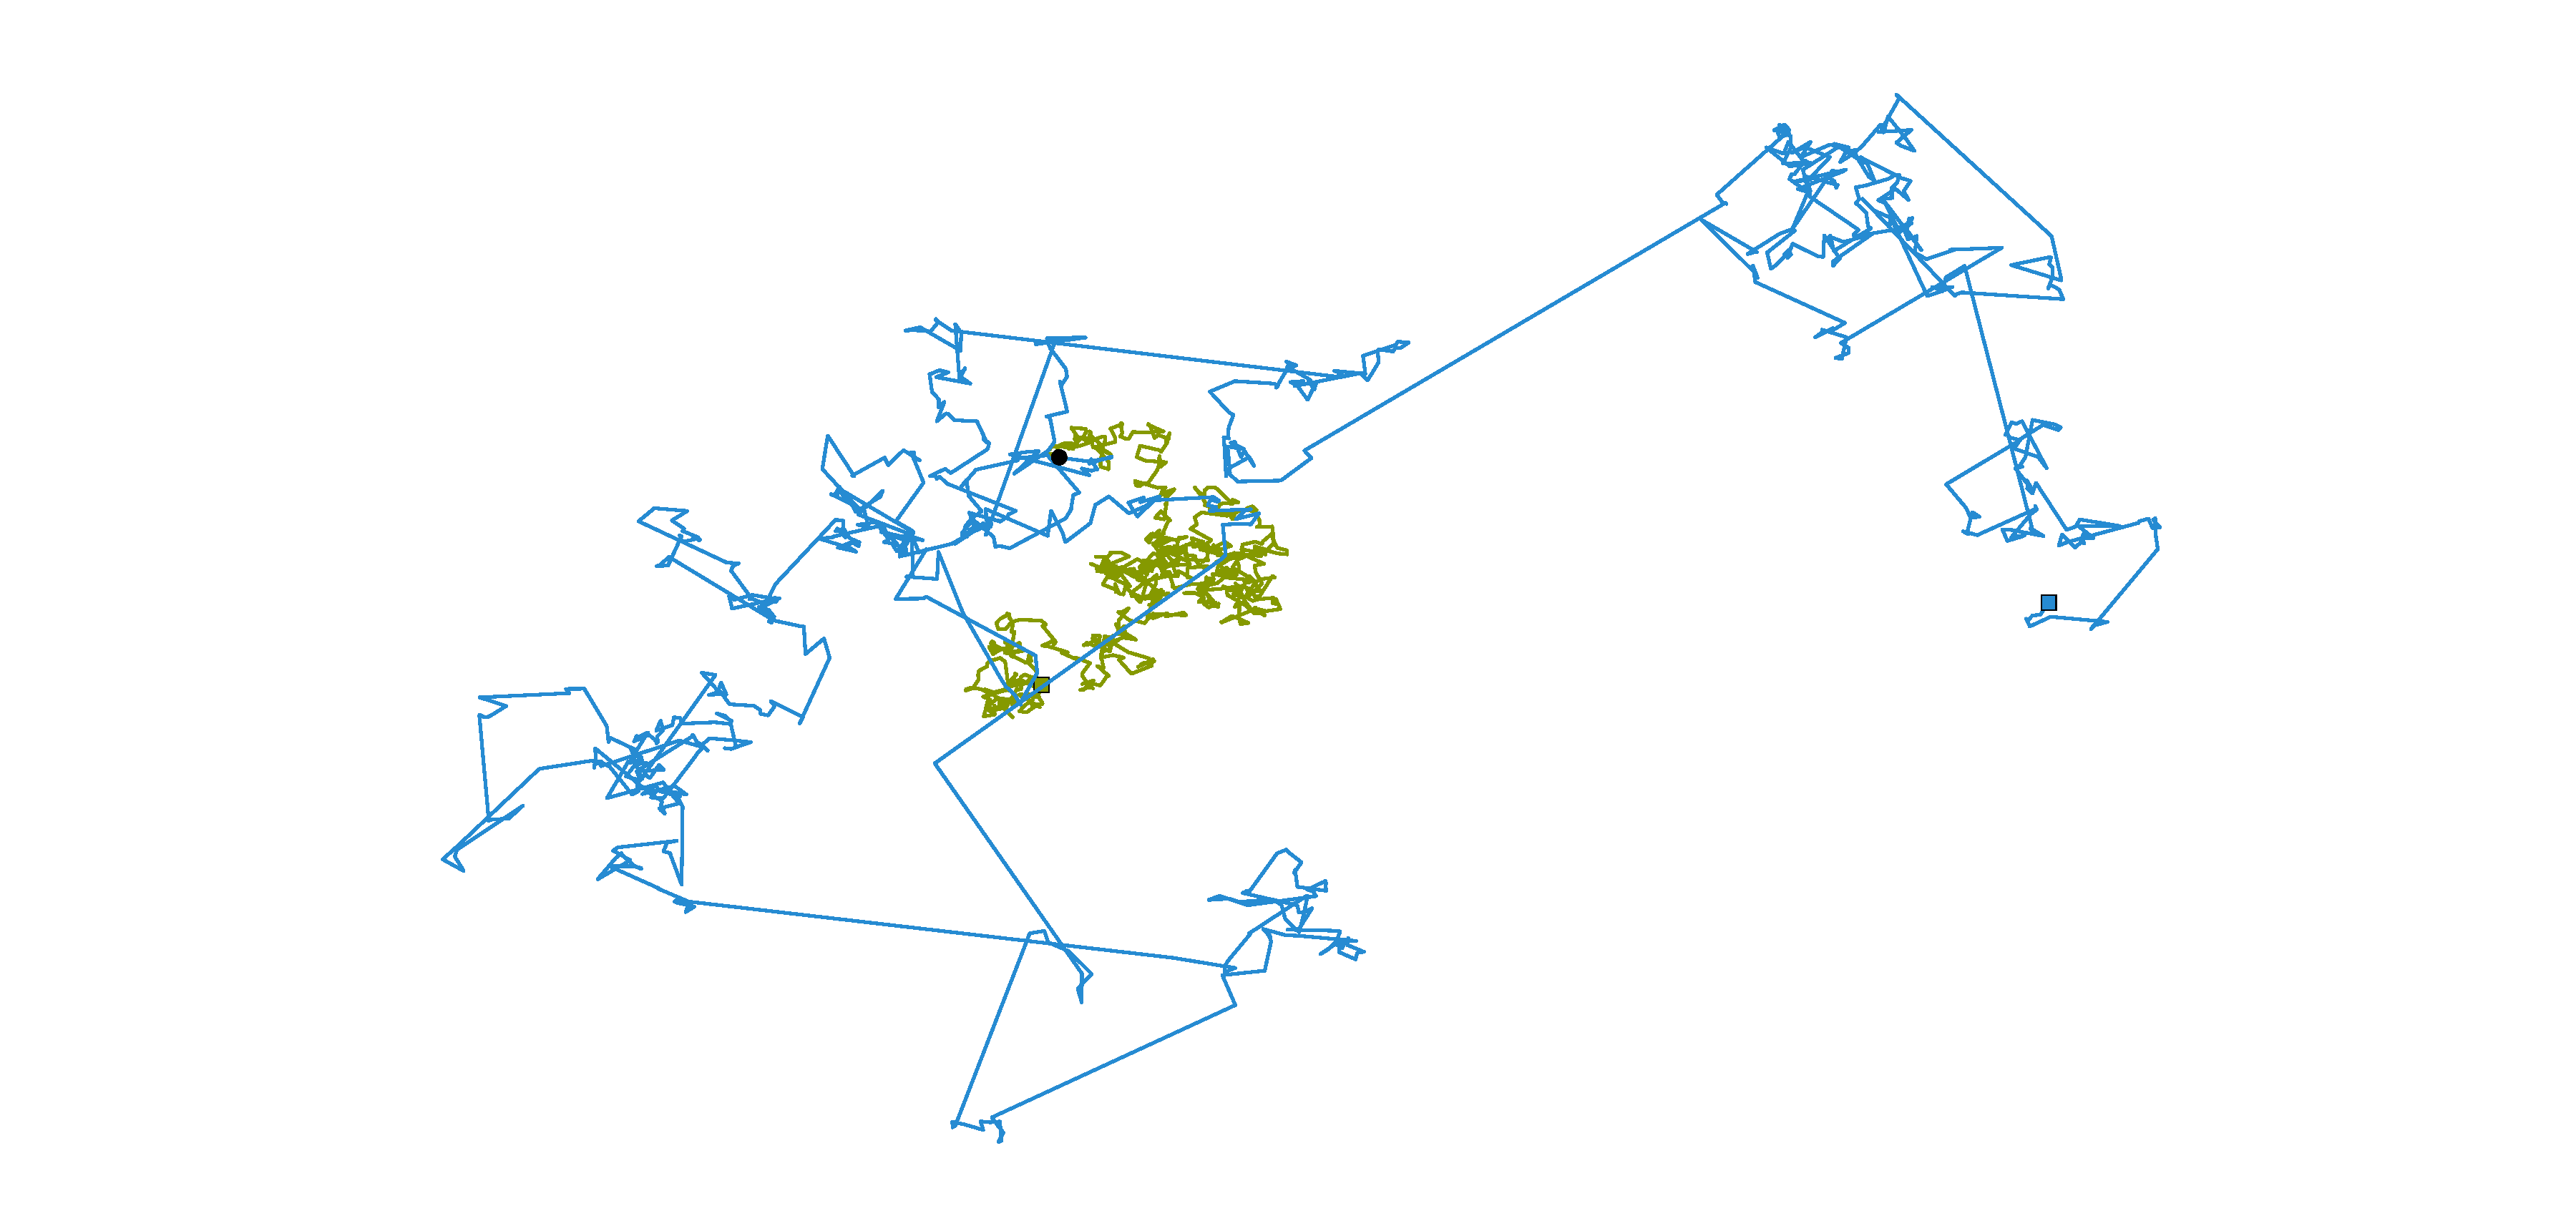
\includegraphics[height=0.4\textheight, clip=true, trim=100mm 10mm 100mm 10mm]{Ressources/Images/Optimisation/LevyFlight/levy_vs_gaussian.pdf}}
        \end{column}%
        \begin{column}{0.55\textwidth}
            \raggedleft
            \includegraphics[height=0.8\textheight]{Ressources/Images/Optimisation/ABC/algorithme_complet.pdf}
        \end{column}%
    \end{columns}%
    \vfill
\end{frame}




% ------------------------------------------------------------------------------
\subsection{Réduction de la complexité}
\begin{frame}[t]
    \addsubtitle{Criblage de Morris}
    \vfill
    \centering
    \begin{columns}
        \begin{column}{0.5\textwidth}
            \centering
            \includegraphics[width=0.6\textwidth]{Ressources/Images/Sensibilite/cube_morris.pdf}
        \end{column}%
        \begin{column}{0.6\textwidth}
            \raggedright
            \uncover<2->{%
            \begin{subequations}
                \begin{align*}
                    \mu^{*} &= \sum_{r = 1}^{R} \frac{\lvert EE_{r} \rvert}{R} \\
                    \sigma &= \sqrt{\sum_{r=1}^{R}\frac{(EE_{r} - \mu)^{2}}{R}}
                \end{align*}
            \end{subequations}
            }
        \end{column}%
    \end{columns}%
    \vfill
    \begin{itemize}
        \item Création d’un plan OAT (One (factor) At the Time).
        \item Évaluation des Effets Élémentaires ($EE$) pour $R$ trajectoires sur $z$ niveaux.
    \end{itemize}
    \vfill
\end{frame}


\begin{frame}[t]
    \addsubtitle{Modèle de substitution par chaos polynomial}
    \vfill
    \centering
    \textbf{Approximation des objectifs par des fonctions analytiques}
    \begin{columns}
        \begin{column}{0.5\textwidth}
            \begin{itemize}
                \item $Conso_{app}$
                \item $Conso_{app}^{CH}$
            \end{itemize}
        \end{column}
        \begin{column}{0.5\textwidth}
            \begin{itemize}
                \item $Conso_{app}^{ECS}$
                \item $Conso_{ref}^{CH}$
            \end{itemize}
        \end{column}
    \end{columns}

    \vfill

    \uncover<2->{%
    \begin{columns}
        \begin{column}{0.6\textwidth}
            \raggedright
            \begin{subequations}
                \begin{align*}
                    &Y = \mathcal{M}(\,\underline{\vec{x}}\,) \approx \sum_{\abs{\vec{\alpha}} \leq P}
                    c_{\vec{\alpha}} \times \psi_{\vec{\alpha}}(\,\underline{\vec{x}}\,) \\
                    \shortintertext{Avec}
                    &\psi_{\vec{\alpha}}(\,\underline{\vec{x}}\,) = \prod_{j = 1}^{D}\pi_{\vec{\alpha}p}^{(j)} \left(\,\underline{x}_{j} \right)
                \end{align*}
            \end{subequations}
        \end{column}
        \begin{column}{0.4\textwidth}
            \centering
            \includegraphics[width=0.8\textwidth]{Ressources/Images/Logos/python_logo.png}
            \includegraphics[width=0.3\textwidth]{Ressources/Images/Logos/openturns.png}
        \end{column}
    \end{columns}
    }
    \vfill
\end{frame}




% % ==============================================================================
% % ==============================================================================
\section{\scshape Application}
% ----------------------------


% ------------------------------------------------------------------------------
\subsection{Conditions limites de l’étude}
\begin{frame}[t]
    \centering
    \textbf{Deux climats étudiés}
    \vfill
    \begin{columns}
        \begin{column}{0.5\textwidth}
            \addsubtitle{Bordeaux}
        \end{column}
        \begin{column}{0.5\textwidth}
            \addsubtitle{Strasbourg}
        \end{column}
    \end{columns}
    \vfill
    \includegraphics[width=0.95\textwidth]{Ressources/Images/EtudeDeCas/irradiations_climats.pdf}
    \vfill
\end{frame}


% ------------------------------------------------------------------------------
\subsection{Réduction de la cardinalité}
\begin{frame}[t]
    \vfill
    \centering
    \includegraphics[width=0.7\textwidth, clip=true, trim=0mm 178mm 0mm 0mm]{Ressources/Images/chapitre3_bilan.pdf}
    \vfill
\end{frame}

\begin{frame}[c]
    \vfill
    \centering
    \begin{columns}
        \begin{column}{0.8\textwidth}
            \uncover<2->{%
                \includegraphics[height=0.9\textheight]{Ressources/Images/Sensibilite/graphInfluence.pdf}
            }
        \end{column}
        \begin{column}{0.2\textwidth}
            \centering
            \small
            \addsubtitle{A priori}
            21 facteurs \\
            \vskip4em
            \uncover<3->{%
            \addsubtitle{Bordeaux}
            $14$ facteurs \\
            \vskip2em
            \addsubtitle{Strasbourg}
            $15$ facteurs
            }
        \end{column}
    \end{columns}
    \vfill
\end{frame}


% ------------------------------------------------------------------------------
\subsection{Création des méta-modèles}
\begin{frame}[t]
    \vfill
    \centering
    \includegraphics[width=0.7\textwidth, clip=true, trim=0mm 128mm 0mm 53mm]{Ressources/Images/chapitre3_bilan.pdf}
    \vfill
\end{frame}

\begin{frame}[c]
    \vfill
    \includegraphics[height=0.3\textheight]{Ressources/Images/Soutenance/Application/meta_results.png}
    \vfill
    \uncover<2->{\includegraphics[width=\textwidth, clip=true, trim=0mm 100mm 0mm 0mm]{Ressources/Images/MetaModele/validite_meta_ssc_600.pdf}}
    \vfill
\end{frame}



% ------------------------------------------------------------------------------
\subsection{Optimisation multi-objectifs}
\begin{frame}[t]
    \vfill
    \centering
    \includegraphics[width=0.7\textwidth, clip=true, trim=0mm 77mm 0mm 53mm]{Ressources/Images/chapitre3_bilan.pdf}
    \vfill
\end{frame}


\begin{frame}[c]
    \addsubtitle{Résultats d’optimisation sur Strasbourg}
    \vfill
    \includegraphics[width=\textwidth]{Ressources/Images/EtudeDeCas/Strasbourg_front_nb_capteurs.pdf}
    \vfill
\end{frame}


\begin{frame}[c]
    \addsubtitle{Occurrences de tailles pour les deux ballons du SSC}
    \vfill
    \centering
    \includegraphics[width=\textwidth]{Ressources/Images/EtudeDeCas/tanks_count.pdf}
    \vfill
\end{frame}


\begin{frame}[c]
    \addsubtitle{SSC sur Strasbourg en fonction du volume des ballons}
    \vfill
    \centering
    \begin{adjustwidth}{-2em}{-2em}
        \includegraphics[width=1.14\textwidth]{Ressources/Images/EtudeDeCas/strasbourg_tanks_variations_cum.pdf}
    \end{adjustwidth}
    \vfill
\end{frame}


% ------------------------------------------------------------------------------
\subsection{Aide à la décision}
\begin{frame}[t]
    \vfill
    \centering
    \includegraphics[width=0.7\textwidth, clip=true, trim=0mm 0mm 0mm 53mm]{Ressources/Images/chapitre3_bilan.pdf}
    \vfill
\end{frame}


\begin{frame}[c]
    \vfill
    \centering
    \only<1-2>{%
        \includegraphics[width=0.7\textwidth]{Ressources/Images/EtudeDeCas/AideDecision/base.png}
        \uncover<2>{\includegraphics[width=0.7\textwidth]{Ressources/Images/EtudeDeCas/AideDecision/volume_ballons.png}}
    }
    \only<3-4>{%
    \uncover<3->{\includegraphics[width=0.7\textwidth]{Ressources/Images/EtudeDeCas/AideDecision/volume_ballons.png}}
    \uncover<4->{\includegraphics[width=0.7\textwidth]{Ressources/Images/EtudeDeCas/AideDecision/final.png}}
    }
    \vfill
\end{frame}














% % ==============================================================================
% % ==============================================================================
\section{\scshape Conclusions / Perspectives}
% ------------------------------------------


% ------------------------------------------------------------------------------
\subsection{Conclusions}
\begin{frame}[c]
    \vfill
    \begin{itemize}
        \item Développements~:
        \begin{itemize}
            \item[--] Modèle de SSC avec une logique de contrôle détaillée.
            \item[--] Algorithme d’optimisation nécessitant très peu de paramètres.
        \end{itemize}
        \vfill
        \uncover<2->{%
        \item Application~:
        \begin{itemize}
            \item[--] Exploration automatisée de l’espace de décision.
            \item[--] Grande diversité de solutions optimales obtenue.
            \item[--] Aide à la décision simple et interactive.
        \end{itemize}
        }
        \vfill
        \item<3-> Mise en évidence du potentiel des SSC pour des MEPOS en climats rudes.
    \end{itemize}
    \vfill
\end{frame}


% ------------------------------------------------------------------------------
\subsection{Perspectives à court terme}
\begin{frame}[c]
    \vfill
    \begin{itemize}
        \item Validation expérimentale du modèle de SSC.
    \vfill
        \item<2-> Prise en compte de l’aspect économique et de l’évolution du climat.
    \vfill
        \item<3-> Incorporation de méthodes de propagation d’incertitudes.
    \vfill
        \item<4-> Ajout de modèles stochastiques pour le comportement des occupants.
    \end{itemize}
    \vfill
\end{frame}


% ------------------------------------------------------------------------------
\subsection{Perspectives à long terme}
\begin{frame}[c]
    \vfill
    \begin{itemize}
        \item Application à la réhabilitation lourde.
    \vfill
        \item<2-> Application aux habitats groupés et aux petits collectifs.
    \end{itemize}
    \vfill
\end{frame}












% % % % % % % % % % % % % % % % % % % % % % % % % % % % % % % % % % % % % % % %
\end{document}
% % % % % % % % % % % % % % % % % % % % % % % % % % % % % % % % % % % % % % % %



% % ==============================================================================
% % ==============================================================================
